%!TEX root =/Users/ludovicl/Dropbox/Cours/UTBM/P15/RapportStage/main.tex


\chapter{Présentation de l'entreprise}


Tech4Team est une startup fondée en juillet 2013 par deux entrepreneurs. Elle propose aujourd'hui deux produits majeurs Inventor-e et Arenametrix.

\section{Inventor-e}
Inventor-e est un logiciel de gestion de planning, de suivi d’états des lieux et de pilotage de maintenance. Il est conçu pour les infrastructures sportives et culturelles multifonctions.

Le logiciel fonctionne sur le principe de client-serveur. L'utilisateur utilise une tablette Android pour faire un état des lieux ou visualiser son planning. Les photos et autres données sont ensuite synchronisées dans une base de données sur un serveur distant. Il est alors possible pour l'utilisateur de visualiser les informations depuis un portail web.

\begin{center}

\includegraphics[scale=0.7]{images/inventore.png}
\captionof{figure}{Principe de fonctionnement d'inventor-e}
\label{inventore}
\end{center}

D'une manière plus technique l'application est développée pour Android 4.0 ou ultérieur, la base de données utilise PostegreSQL et l'interface web est développée avec le framework Ruby on Rails.

\section{Arenametrix}
Arenametrix est une solution logicielle, flexible, clé en main et intégrée de Big Data (analyse et exploitation des données billetteries), disponible en SaaS, pour la connaissance et la fidélisation des publics, la prospection ciblée et la mise en place d'une nouvelle politique de tarification

ArenaMetrix de décompose en trois briques technologiques indépendantes ou combinées : 
\begin{itemize}
  \item[\textbullet] ArenaPublic : Socle e-CRM
  \item[\textbullet] ArenaProspection : Prospection ciblée
  \item[\textbullet] ArenPricing : Tarification dynamique
\end{itemize}

\begin{center}
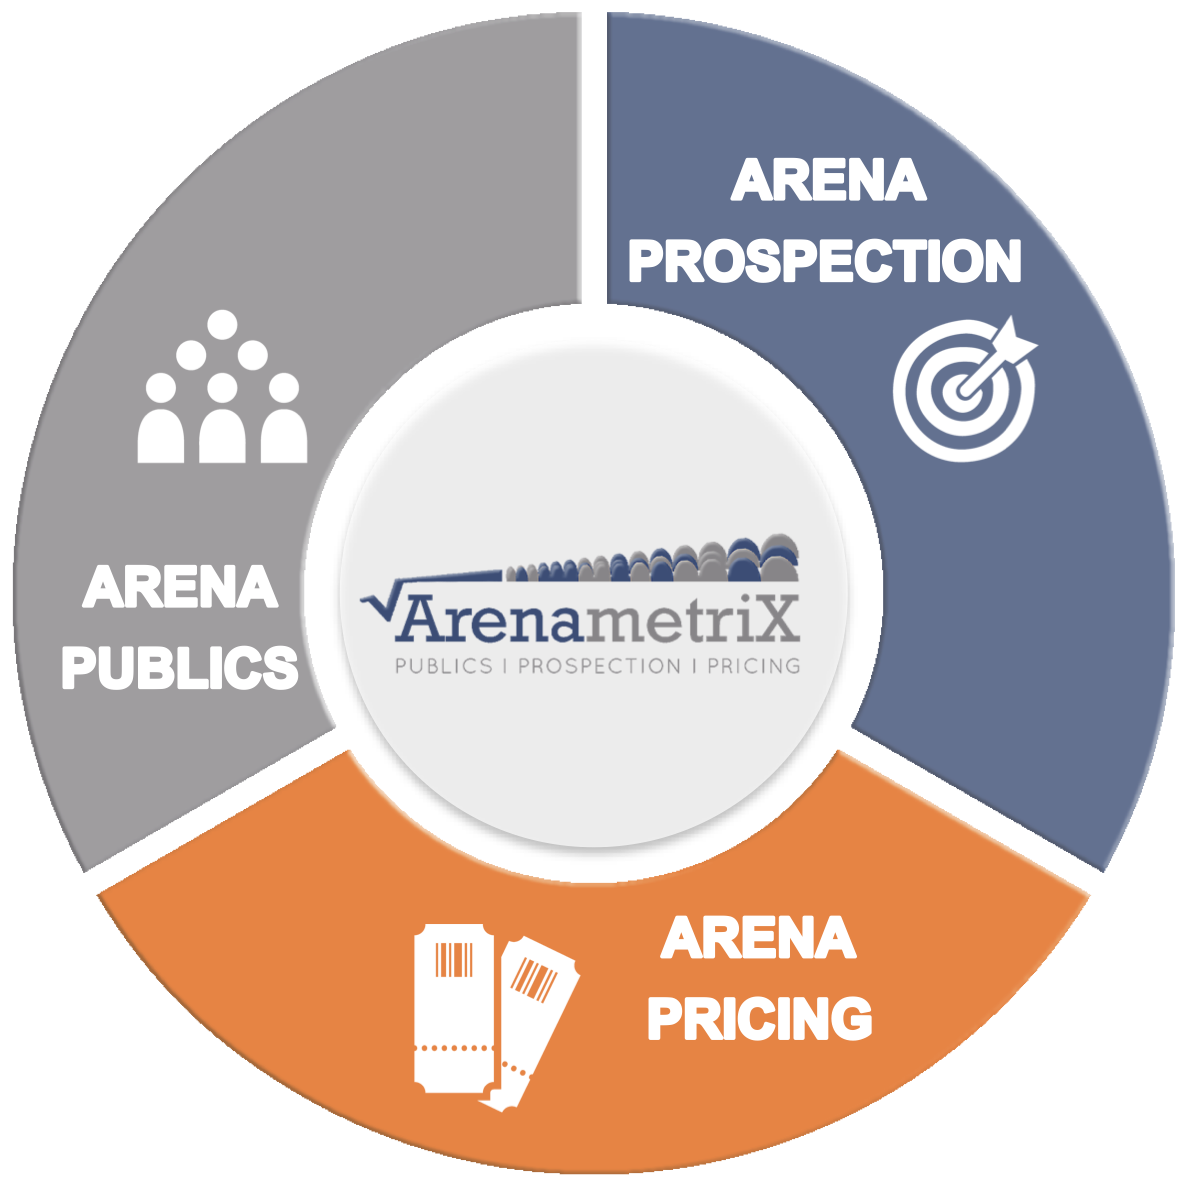
\includegraphics[scale=0.45]{images/arenametrix.png}
\captionof{figure}{Vision à 360\ensuremath{^\circ}  de Arenametrix}
\label{arenametrix}
\end{center}

\subsection{ArenaPublic}
ArenaPublic est le socle e-CRM d’exploitation des données publics.

Il permet :
\begin{itemize}
  \item[\textbullet] La centralisation des données publiques, B to B et B to C
  \item[\textbullet] Le nettoyage et enrichissement des données (sexe, âge, lieu de résidence, fréquentation du stade, dépenses merchandising…)
  \item[\textbullet] La visualisation graphique de la base de données à 360\ensuremath{^\circ}
  \item[\textbullet] L'analyse mono variable et bi variable en croisant des données identitaires et de consommation
\end{itemize}

\subsection{ArenaProspection}
Module d’optimisation du démarchage commercial.

Ce module permet :
\begin{itemize}
  \item[\textbullet] La sélection d’une liste de contacts
  \item[\textbullet] Le classement des prospects selon leur probabilité de souscription
  \item[\textbullet] La gestion interfacée d’une campagne de téléprospection, de mailing et de SMS auprès des prospects
  \item[\textbullet] L'analyse des retours : réaction au démarchage, taux de conversion et intégration à la priorisation
\end{itemize}

\subsection{ArenaPricing}
Module de yield management.

Ce module permet :
\begin{itemize}
  \item[\textbullet] La création de typologies de publics par segmentation et profilage
  \item[\textbullet] La prévision de la demande en billets pour un événement
  \item[\textbullet] Recommandations tarifaires en fonction de la date et de la catégorie
  \item[\textbullet] La gestion des flux par le prix, en transparence avec le client final
\end{itemize}

\subsection{Objectifs}
Tech4Team prévoir plusieurs objectifs pour son produit :
\begin{itemize}
	\item[\textbullet] Démocratisation de l'accès à la culture en ouvrant la voie à des prix différenciés
	\item[\textbullet] Stabilisation voir hausse de la rentabilité des structures culturelles en augmentant le chiffre d'affaires billereterie de 5 à 7\%
\end{itemize}

\section{Fonctionnement de l'entreprise et répartition des tâches}
Durant la majeure partie de mon stage l'équipe se composé de six stagiaires, cinq en développement et un commercial, un développeur expérimenté en cdi et les deux fondateurs. \\

Sur Arenametrix : 
\begin{itemize}
  \item[\textbullet] Un stagiaire s'occupait du front-end et de l'affichage des données
  \item[\textbullet] Un stagiaire s'occupait de la partie analyse de données
  \item[\textbullet] Un stagiaire s'occupait du scoring
  \item[\textbullet] Le développeur en cdi validait nos choix techniques sur le produit et jouait également le rôle d'administrateur système
  \item[\textbullet]Moi, je m'occupais du back-end et de l'importation des données
\end{itemize} \

Sur Inventor-e : 
\begin{itemize}
  \item[\textbullet] Un stagiaire s'occupait de l'application Android
  \item[\textbullet] Le développeur en CDI s'occupait de la base de données et de l'interface web
\end{itemize}

\leavevmode
\\
Les deux fondateurs s'occupaient des relations clients avec le commercial et nous attribuaient des tâches pour améliorer et faire évoluer les produits. Des réunions sont régulièrement organisées pour définir les architectures logiciels, de base de données et les moyens techniques à utiliser. 
\\ 

La gestion de projets se fait avec l'outil open source Redmine. Pour la gestion du code source, nous utilisons Git et la plateforme Gitlab.

\subsection{Organigramme de l'entreprise a la fin de mon stage}
Comme le montre la figure \ref{organigramme} page \pageref{organigramme}, à la fin de mon stage nous étions 13 dans l'entreprise. 

\begin{itemize}
  \item[\textbullet] Le lead développeurs est en CDI depuis 1 an, il s'occupe de toute la partie technique de l'entreprise, que ce soit pour Inventor-e en développement activement l'application web et pour ArenaMetrix mais de manière plus macro.

  \item[\textbullet] Le directeur du développement est en CDI, recruté récemment il s'occupe de faire le lien entre les clients et les développeurs.

  \item[\textbullet] Le responsable mobile est un ancien stagiaire passé en CDD, il s'occupe de l'application Android d'Inventor-e.
  
  \item[\textbullet] Le responsable front-end est un ancien stagiaire, il a terminé son stage 1 mois avant moi et est maintenant en CDD
  
  \item[\textbullet] Moi qui suis maintenant responsable de la partie back-end, j'ai signé un CDI a la fin de mon stage.
  
  \item[\textbullet] Les deux data scientist, un va signer un CDI à la fin de son stage et l'autre doit faire de l'alternance dans une autre entreprise
  
          
  \item[\textbullet]Les autres développeurs et la responsable marketing et communication sont des stagiaires pour 6 mois. 

\end{itemize}

\begin{center}
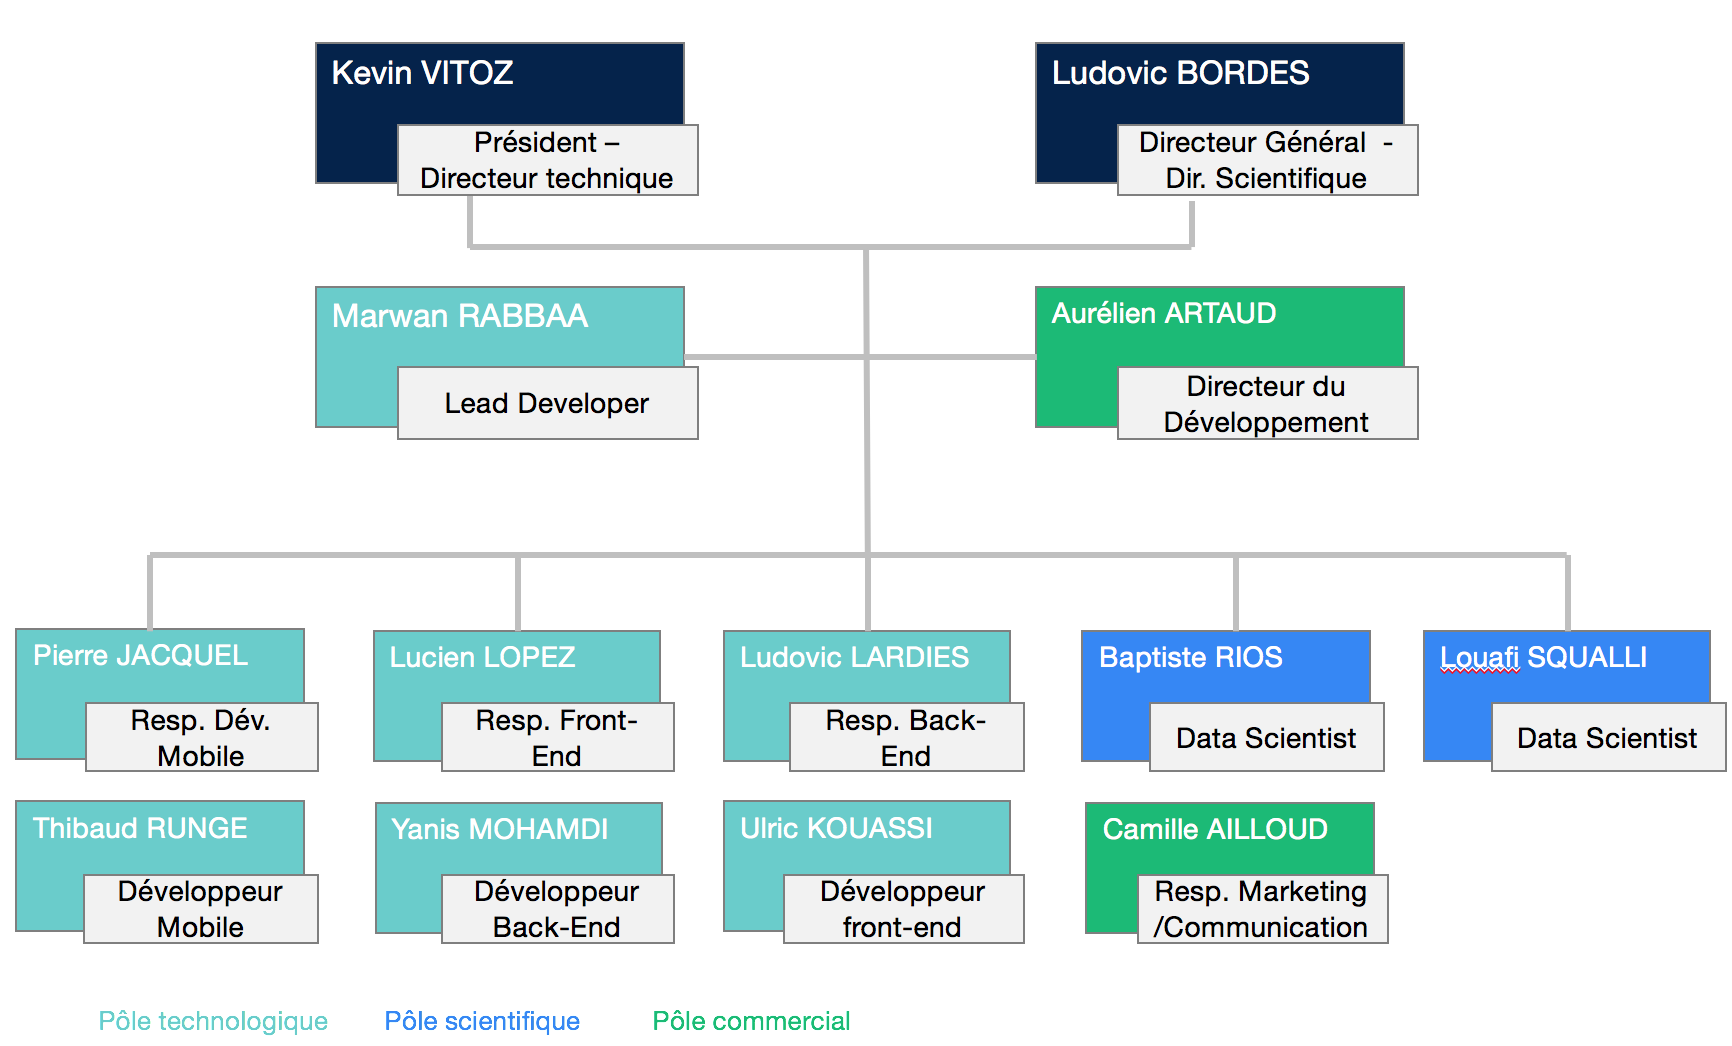
\includegraphics[scale=0.57]{images/organigamme.png}
\captionof{figure}{Organigramme de l'entreprise}
\label{organigramme}
\end{center}


